\chapter{Воздушные суда и их производители}%
\label{ch:aircraft-chapter}

Глава посвящена исследованию различных свойств воздушных судов на основе базы Викиданные. 
В ходе исследования с помощью SPARQL-запросов, вычисляемых на объектах типа <<Воздушные суда>>, 
получен список воздушных судов и их производителей, получено число выпущенных самолётов для разных моделей. Для этого числа самолётов по моделям проверено выполнение \href{https://w.wiki/vDs}{закона Парето}. 
Также получена диаграмма, отражающая соотношение общего количества производителей воздушных судов по странам. 
В заключении главы получена оценка полноты данных, представленных в Википедии и Викиданных. Согласно ей в Викиданных представлено всего 595 записей о производителей воздушных судов из \num{1700} на 2020 год.
Если считать, что ежегодно будет появляться фиксированное количество новых авиапроизводителей и количество ежегодно заносимых записей в Викиданные останется неизменным, то можно предположить, что примерно через 75 лет (то есть в 2095 году) Викиданные будут содержать записи обо всех авиапроизводителях.

\section{Список самолётов}

Воздушное судно~--- летательный аппарат, поддерживаемый в атмосфере за счёт взаимодействия с воздухом, отличного от взаимодействия с воздухом, отражённым от поверхности земли или воды.
К воздушным судам относятся следующие виды летательной техники: автожир, аэростат, вертолёт, винтокрыл, дирижабль, махолёт, планёр и самолёт.
К воздушным судам не относятся космические корабли, ракеты, экранопланы (но не экранолёты) и суда на воздушной подушке. 

Построим список всех экземпляров объекта <<Воздушные суда>> \href{https://www.wikidata.org/wiki/Q11436}{Q11436}.

%\begin{itemize}
%\itemОбъект: Воздушное судно (Q11436).
%\itemСвойство: Экземпляр (P31).
%\end{itemize}

\begin{lstlisting}[ language=SPARQL, caption={\href{https://w.wiki/t3j}{Список воздушных судов}\protect\footnotemark}, label=lst:lang1, ]
#List of `instances of` "aircraft"
SELECT ?plane ?planeLabel
WHERE
{
    ?plane wdt:P31 wd:Q11436. # instances of aircraft
    SERVICE wikibase:label { bd:serviceParam wikibase:language "ru" }
}
\end{lstlisting}
\footnotetext{Получено 153 воздушных судна в 2017 году, 299 воздушных судов в 2020 году. Ссылка на SPARQL-запрос: \href{https://w.wiki/t3j}{https://w.wiki/t3j}}

%Результатом запроса~\ref{lst:lang1} (на английском языке) является список всех воздушных судов. На 2017 год список содержал \num{1564} записи, а к 2020 году число записей увеличилось до \num{3325}.
%На руском языке на 2017 год результат запроса~\ref{lst:lang1} содержал 153 записи, а к 2020 году их число увиличилось до 299 записей.

Наиболее полными и проработанными воздушными судами на Викиданных на 2017 год являются: \href{https://www.wikidata.org/wiki/Q271446}{МиГ-3}, \href{https://www.wikidata.org/wiki/Q1349098}{Як-36}, \href{https://www.wikidata.org/wiki/Q429839}{Mitsubishi A5M}. На 2020 год наиболее полными и проработанными воздушными судами на Викиданных являются: \href{https://www.wikidata.org/wiki/Q770863}{Sopwith Triplane} (18 свойств), \href{https://www.wikidata.org/wiki/Q1658673}{Ил-103} (14 свойств) и \href{https://www.wikidata.org/wiki/Q665071}{Martin 2-0-2} (14 свойств).
Количество свойств было получено при помощи сервиса \href{https://prowd.id/dashboards/972cd00ce110/profile}{ProWD} \cite{aircraft_prowd}, который позволяет проанализировать выбранный объект Викиданных.
%Почти пустыми и малоинформативными воздушными судами на 2017 год оказались: \href{https://www.wikidata.org/wiki/Q464247}{МиГ-1}, \href{https://www.wikidata.org/wiki/Q2296502}{Су-6}, \href{https://www.wikidata.org/wiki/Q1658673}{Ил-103}.
На 2020 год малоинформативными воздушными судами являются: \href{https://www.wikidata.org/wiki/Q820603}{Бе-1} (3 свойства), \href{https://www.wikidata.org/wiki/Q117984}{Литуаника} (4 свойства) и \href{https://www.wikidata.org/wiki/Q572762}{Ла-168} (3 свойства).

\section{Производители воздушных судов}

Построим список производителей воздушных судов, выполнив запрос~\ref{lst:lang2}.

\index{SPARQL!COUNT!Производители воздушных судов}
\begin{lstlisting}[ language=SPARQL, caption={\href{https://w.wiki/t3n}{Производители воздушных судов}\protect\footnotemark}, label=lst:lang2, ]
# Count aircraft having property manufacture, group by manufacture
SELECT ?manufacture ?manufactureLabel (COUNT(?plane) AS ?count) 
WHERE {
  ?plane wdt:P31 wd:Q11436.     # instance of aircraft
  ?plane wdt:P176 ?manufacture. # manufacture
  SERVICE wikibase:label { bd:serviceParam wikibase:language "ru". }
}
GROUP BY ?manufacture ?manufactureLabel
\end{lstlisting}
\footnotetext{Получено 300 производителей воздушных судов в 2017 году, 590 производителей воздушных судов в 2020 году. Ссылка на SPARQL-запрос: \href{https://w.wiki/t3n}{https://w.wiki/t3n}}

\marginnote{

У каких из представленных ниже российских производителей самолётов есть веб-сайты?
\begin{itemize}
\item \href{https://w.wiki/vDw}{Миг}
\item \href{https://w.wiki/vDx}{Саратовский авиационный завод}
\item \href{https://w.wiki/vDy}{Туполев}
\item \href{https://w.wiki/vDz}{Сухой}
\end{itemize}
См. ответ~\ref{answer:aircraft_manufacturers} на с.~\pageref{answer:aircraft_manufacturers}.
}

Результатом запроса~\ref{lst:lang2} является список всех производителей воздушных судов с указанием количества различных моделей, производимых данным заводом.

\section{Количество выпущенных воздушных судов}

\index{Самолёты!Определения!Авиационная промышленность}
Авиационная промышленность~--- это одна из самых крупных отраслей машиностроения в мире. 
В её задачи входит как разработка, так и производство различной воздушной техники. 
Для того чтобы оценить, какие модели воздушных судов являются самыми массовыми, 
мы построим диаграмму произведенных судов различных моделей, представленную на рис.~\ref{fig:Number_of_aircraft_produced_ru_2020}. 
Чтобы получить количество произведённых воздушных судов, необходимо выполнить запрос~\ref{lst:lang3}.

\begin{lstlisting}[ language=SPARQL, caption={\href{https://w.wiki/v4J}{Список моделей, упорядоченный по количеству выпущенных самолётов}\protect\footnotemark}, label=lst:lang3, ]
# List of aircraft models, sorted by number of aircraft built
SELECT ?plane ?planeLabel ?planes_produced WHERE {
  ?plane wdt:P31 wd:Q11436. # instance of aircraft
  ?plane wdt:P1092 ?planes_produced.  # total aircraft manufactured
  SERVICE wikibase:label {bd:serviceParam wikibase:language "ru,en".}
}
ORDER BY DESC(?planes_produced)
\end{lstlisting}
\footnotetext{Получено 288 моделей, для которых известно число выпущенных самолётов, 2020 год. Ссылка на SPARQL-запрос: \href{https://w.wiki/v4J}{https://w.wiki/v4J}}

%В результатом запроса~\ref{lst:lang3} мы получили список состоящий из 177 записей (на 2020 год) моделей воздушных судов и их суммарного произведенного количества за всё время.

Некоторые модели воздушных судов были выпущены в единичных экземплярах, поэтому для повышения читабельности диаграммы~\ref{fig:Number_of_aircraft_produced_ru_2020} их можно исключить. Для получения нового списка добавим в запрос~\ref{lst:lang3_1} фильтр по количеству выпущенных самолётов.


\index{SPARQL!FILTER!Список выпущенных самолётов, в количестве более 10 штук}
\begin{lstlisting}[ language=SPARQL, caption={\href{https://w.wiki/v4N}{Список, включающий только те самолёты, которые были выпущены в количестве более 10 штук}\protect\footnotemark}, label=lst:lang3_1, ]
# List of aircraft models, sorted by number of aircraft built
#defaultView:BarChart
SELECT ?plane ?planeLabel ?planes_produced WHERE {
  ?plane wdt:P31 wd:Q11436. # instance of aircraft
  ?plane wdt:P1092 ?planes_produced.  # total aircraft manufactured
  FILTER (?planes_produced > 10)
  SERVICE wikibase:label {bd:serviceParam wikibase:language "ru,en".}
}
ORDER BY (?planes_produced)
\end{lstlisting}
\footnotetext{Получен отфильтрованный по количеству выпущенных самолётов список, состоящий из 124 моделей. Ссылка на SPARQL-запрос: \href{https://w.wiki/v4N}{https://w.wiki/v4N}}

%Итого, результатом запроса~\ref{lst:lang3_1} уже будет 86 записей, а не 177.

\label{aircraft_question_2}
\marginnote{
Найдите соответствие между датой основания и компанией в следующей таблице:
\\
\begin{tabular}{ l | l }
Компания & Дата основания \\ \hline
\href{https://w.wiki/vDw}{Миг} & 1 января 1939 \\
\href{https://w.wiki/vE4}{Вымпел} & 18 ноября 1949 \\
\href{https://w.wiki/vDy}{Туполев} & 18 декабря 1939 \\
\href{https://w.wiki/vDz}{Сухой} & 1 января 1922 \\
\end{tabular}
\\
См. ответ~\ref{answer:aircraft_company_foundation_date} на с.~\pageref{answer:aircraft_company_foundation_date}.
}

На рисунке рис.~\ref{fig:Number_of_aircraft_produced_ru_2020} видно, что на 2020 год больше всего было выпущено воздушных судов следующих моделей: \href{https://www.wikidata.org/wiki/Q2096452}{Piper PA-32} (\num{7842} штук), \href{https://www.wikidata.org/wiki/Q1860367}{Piper PA-24 Comanche} (\num{4857}), \href{https://www.wikidata.org/wiki/Q694521}{Junkers W 34} (\num{3000}), \href{https://www.wikidata.org/wiki/Q4046989}{Piper J-4} (\num{1251}).

%\clearpage
\begin{figure*}[h]

    \setlength{\fboxsep}{0pt}%
    \setlength{\fboxrule}{1pt}%
    \fcolorbox{gray}{gray}{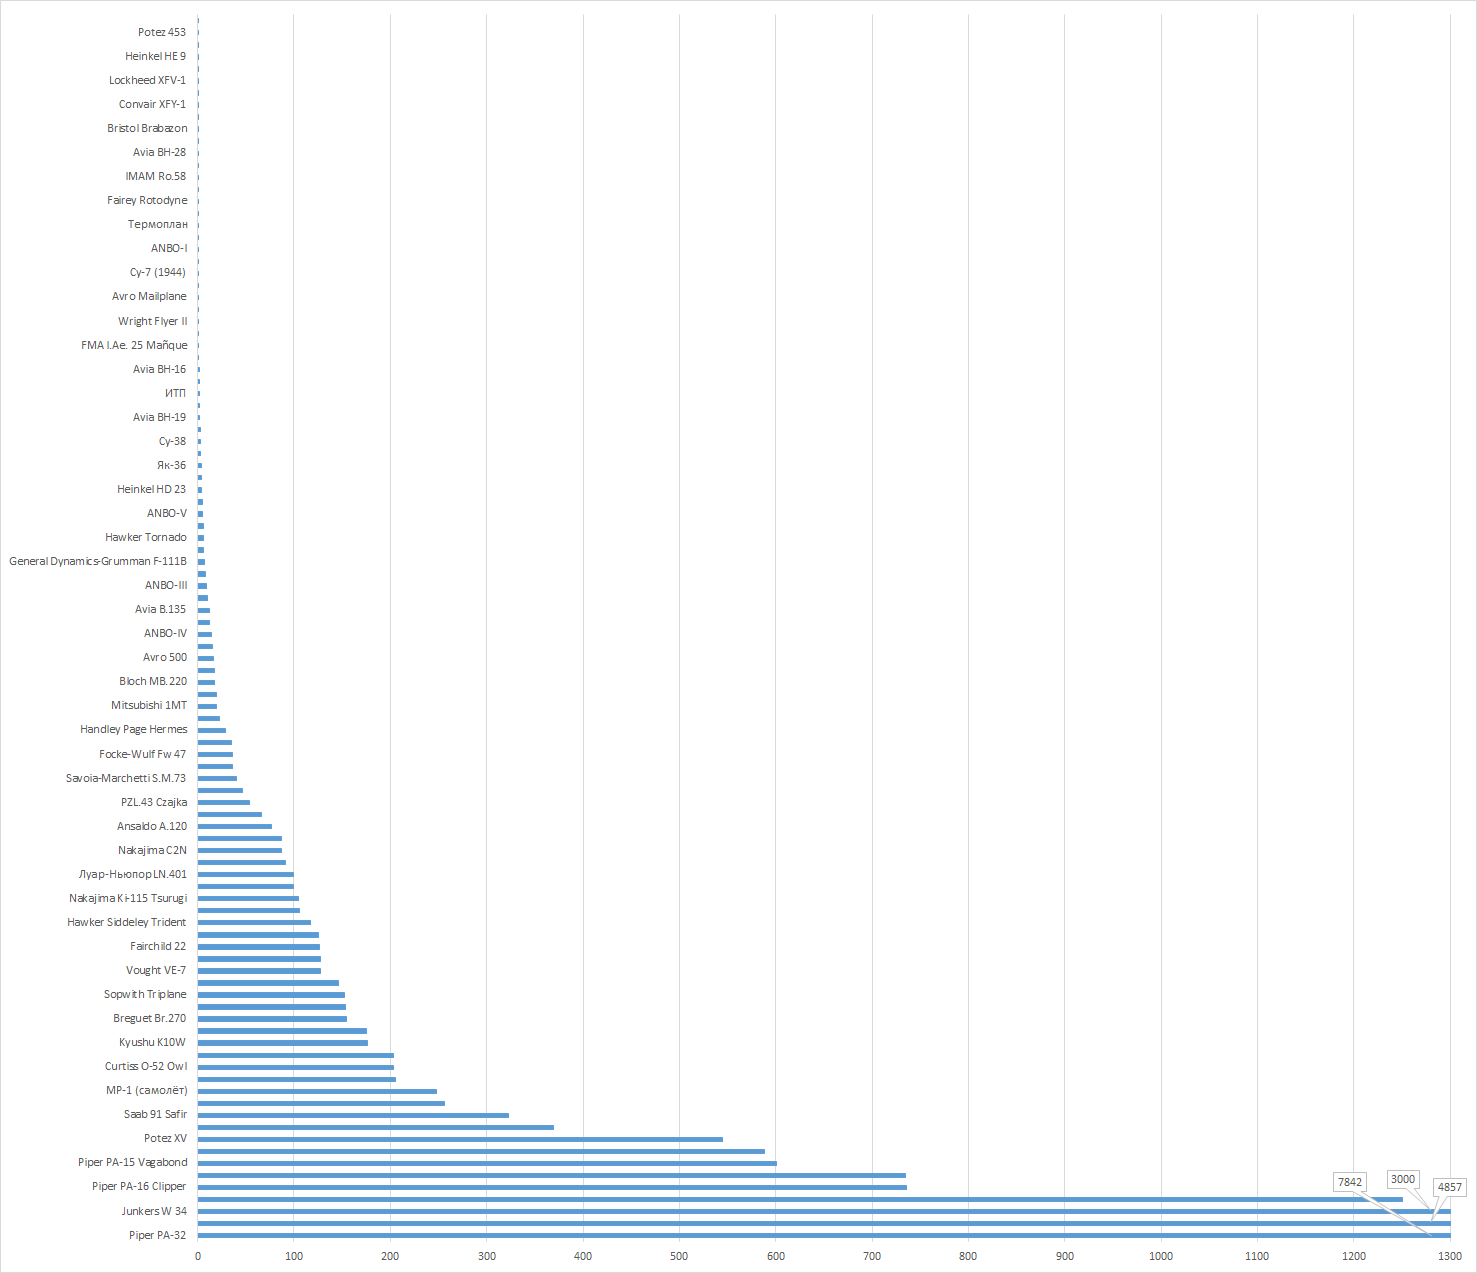
\includegraphics[width=\linewidth]{./chapter/aircraft/Number_of_aircraft_produced_ru.png}}%

%	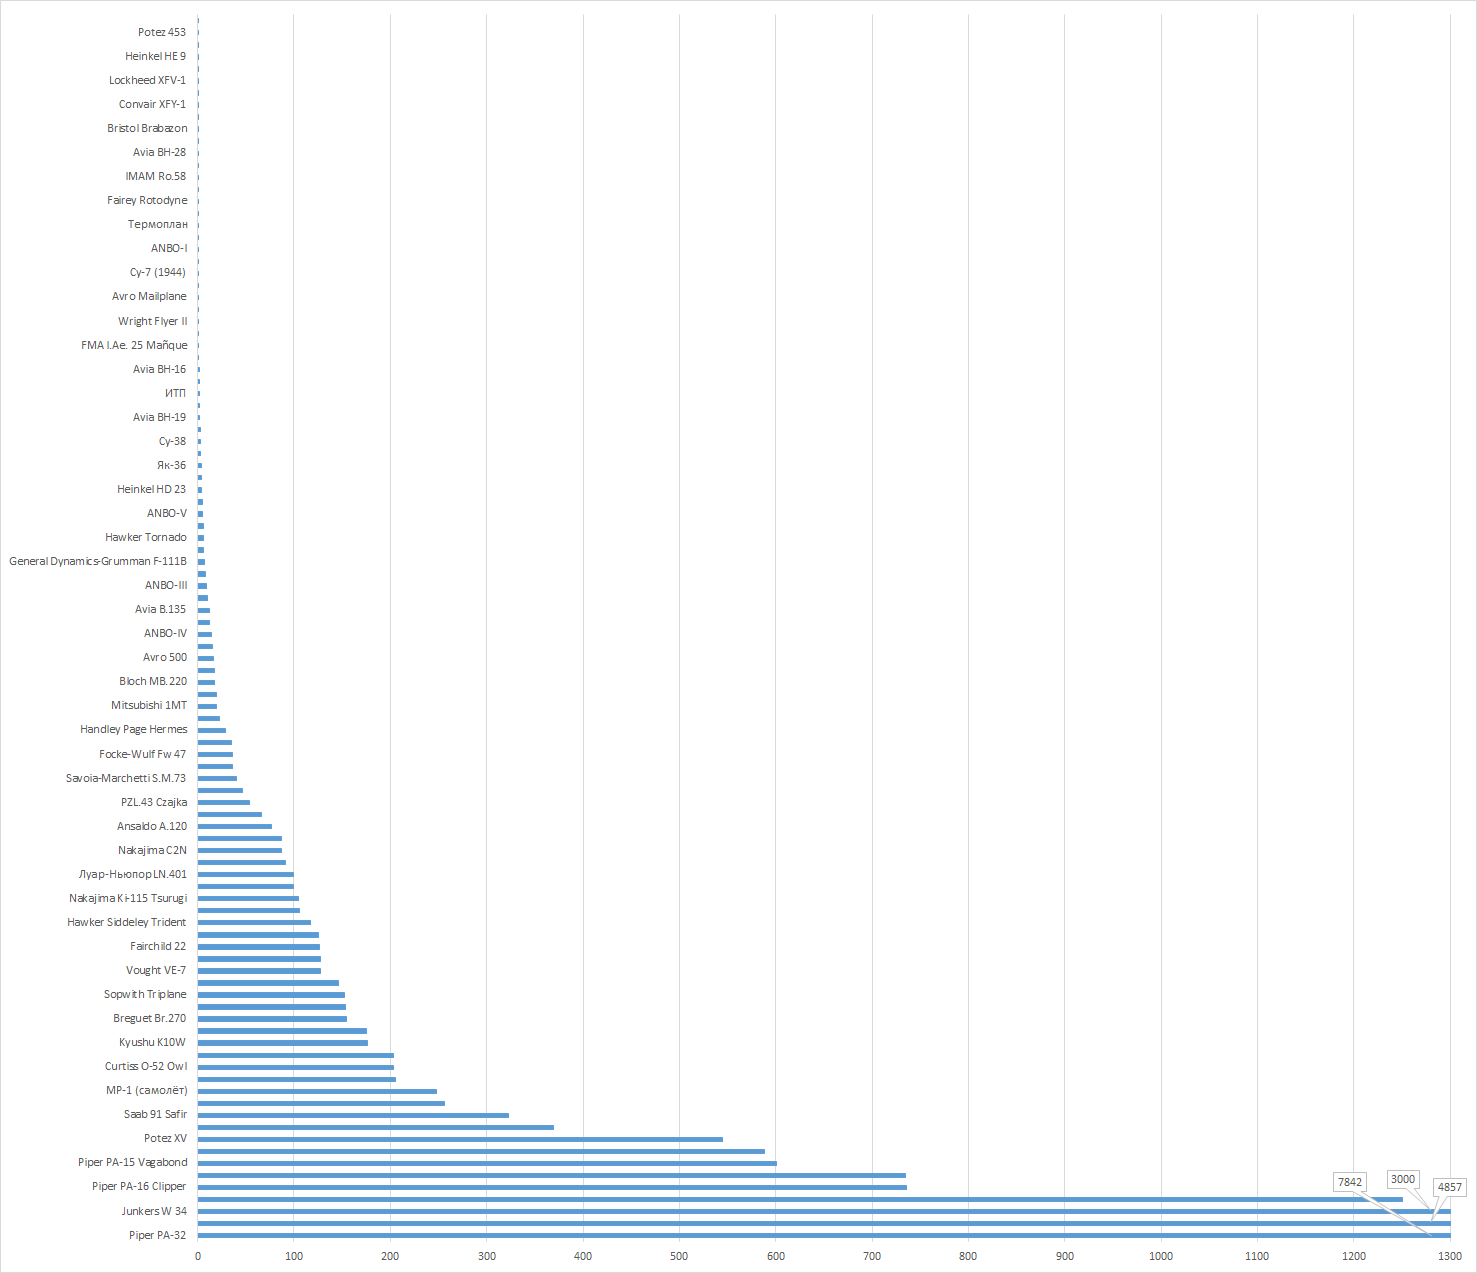
\includegraphics{./chapter/aircraft/Number_of_aircraft_produced_ru.png}%
	\caption{Количество выпущенных воздушных судов по моделям, 2020. Диаграмма построена в Microsoft Excel на основе данных, полученных с помощью запроса~\protect\ref{lst:lang3_1}.}%
    \label{fig:Number_of_aircraft_produced_ru_2020}%
\end{figure*}

%По диаграмме видно, что больше всего было выпущено воздушных судов следующих моделей: Piper PA-32 (\num{7842} штук), Piper PA-24 Comanche (\num{4857}), Junkers W 34 (\num{3000}), Piper J-4 (\num{1251})

\newpage 
\index{Самолёты!Определения!Закон Парето}
Теперь попытаемся ответить на вопрос выполняется ли \href{https://w.wiki/vDs}{Закон Парето} относительно числа моделей самолётов?

Для того чтобы построить график процентного соотношения количества выпущенных моделей самолётов к общему числу произведённых самолётов, необходимо выполнить следующие шаги:

%\footnotetext{Диаграмма~\ref{fig:Number_of_aircraft_produced_ru_2020} была построена в excel на основании данных, полученных из запроса~\ref{lst:lang3_1}}.

\begin{enumerate} 
  \item Подсчитать общее число самолётов по всем моделям, с помощью скрипта~\ref{lst:lang3_2}.
  
  \index{SPARQL!SUM!Общее число произведённых самолётов}
  
\begin{lstlisting}[ language=SPARQL, caption={\href{https://w.wiki/vE9}{Общее число произведённых самолётов}\protect\footnotemark}, label=lst:lang3_2, ]
SELECT (SUM(?count) as ?sum) WHERE {
  SELECT ?count WHERE {
    ?plane wdt:P31 wd:Q11436; # instance of aircraft
		   wdt:P1092 ?count. # total aircraft manufactured
  }
}
\end{lstlisting}
\footnotetext{Общее число выпущенных самолётов на 2020 год составляет \num{44151}. Ссылка на SPARQL-запрос: \href{https://w.wiki/vE9}{https://w.wiki/vE9}}
  
  %В результате выполнения запроса~\ref{lst:lang3_2} мы получили общее число выпущенных самолётов на 2020 год = \num{33177}.
  
  \item По оси Х откладывается число рассматриваемых моделей самолётов (то есть при х = 1 мы рассматриваем число выпущенных самолётов первой модели, при х = 2~--- число выпущенных самолётов первой и второй модели и так далее). По оси Y будем откладывать F(n) = $\sum\limits_{i=1}^n f(i)$, где f(i)~--- число выпущенных самолётов модели i. При этом выполняется условие f(i) > f(j), при i < j, где i, j~--- номер модели самолёта (то есть количество выпущенных моделей самолётов заранее упорядочивается по убыванию). Также по оси Х откладываем вторую шкалу от 0 до 1, чтобы легче было определить параметры для проверки выполнения \href{https://w.wiki/vDs}{закона Парето}.
\end{enumerate}

\begin{figure*}[h]

    \setlength{\fboxsep}{0pt}%
    \setlength{\fboxrule}{1pt}%
    \fcolorbox{gray}{gray}{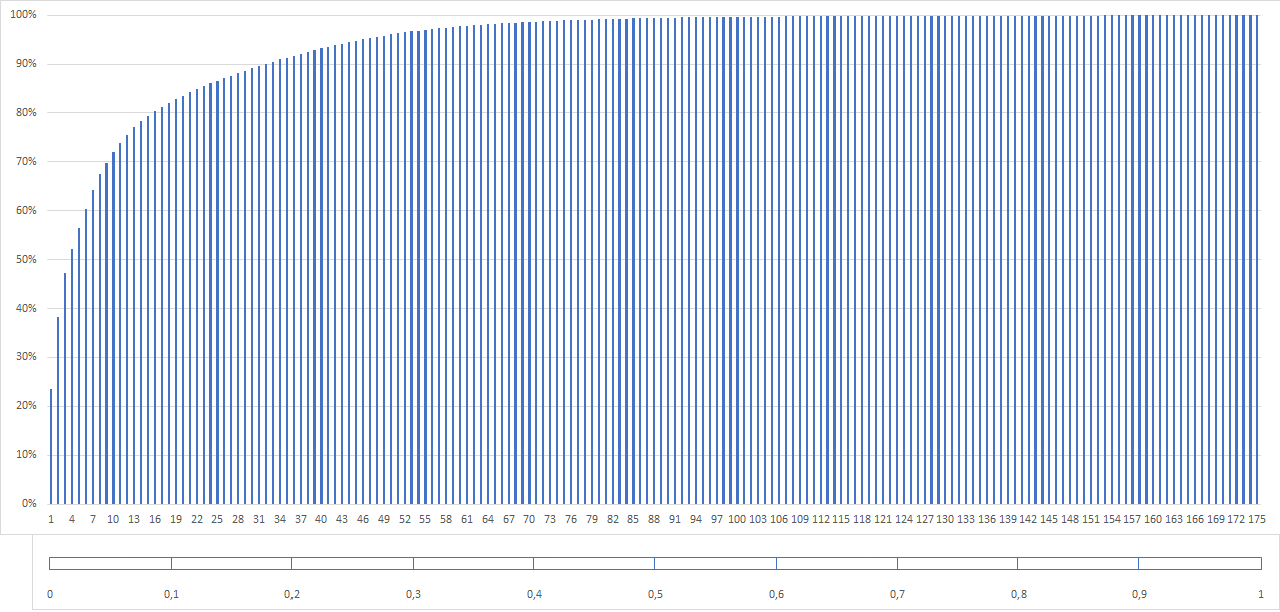
\includegraphics[width=\linewidth]{./chapter/aircraft/Pareto_principle_diargam.png}}%

%	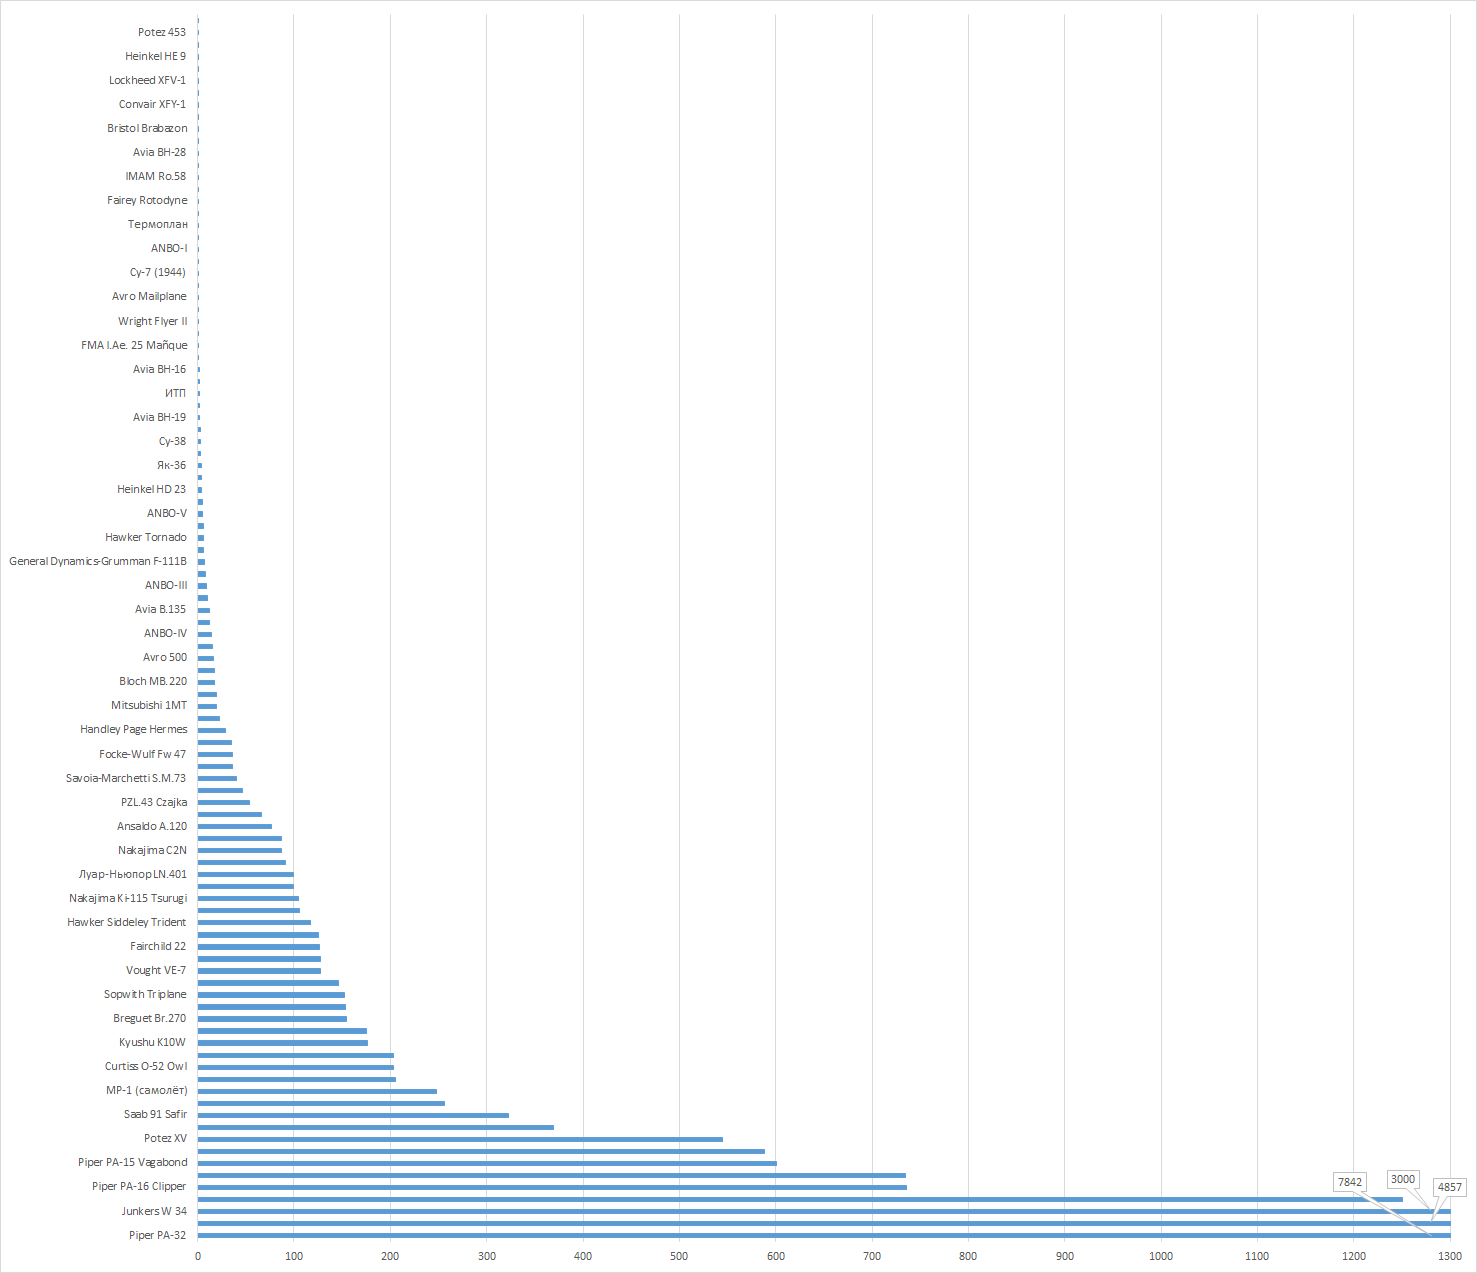
\includegraphics{./chapter/aircraft/Number_of_aircraft_produced_ru.png}%
	\caption{Процентное соотношение количества выпущенных моделей самолётов по n моделям к общему числу выпущенных самолётов за всё время, 2020.}%
    \label{fig:Pareto_principle_diargam}%
\end{figure*}

\index{Самолёты!Определения!Закон Парето}
По графику~\ref{fig:Pareto_principle_diargam} видно, что 80\% всех выпущенных самолётов приходится на 16 различных моделей самолётов, что составляет 9,2\% от общего числа моделей. Закон Парето утверждает, что: \href{https://w.wiki/vDs}{«20\% усилий дают 80\% результата, а остальные 80\% усилий — лишь 20\% результата»}. Можно сделать вывод, что выполняется более сильный закон, чем принцип Парето относительно числа моделей самолётов.
\footnotetext{Закон Парето: \href{https://w.wiki/vDs}{https://w.wiki/vDs}}

\section{В каких странах производят самолёты}

\label{aircraft_question_3}
\marginnote{
Найдите соответствие между расположением штаб-квартиры компании и названием компании производителя самолётов в следующей таблице:
\\
\begin{tabular}{ l | l }
Компания & Штаб-квартира \\ \hline
\href{https://w.wiki/vEP}{Камов} & Улан-Удэ \\
\href{https://w.wiki/vER}{Авиадвигатель} & Пермь \\
\href{https://w.wiki/vEL}{Улан-Удэнский завод} & Москва \\
\href{https://w.wiki/vDz}{Сухой} & Люберцы \\
\end{tabular}
\\
См. ответ~\ref{answer:aircraft_company_headquarters} на с.~\pageref{answer:aircraft_company_headquarters}.
}

Построим список количества производителей воздушных судов по странам. Для выполнения запроса~\ref{lst:lang5} используем группировку по странам (GROUP BY) и при помощи функции Count() для каждой страны подсчитаем общее количество авиастроительных заводов.

%\index{SPARQL!COUNT!Список соотношения количества производителей воздушных судов по странам}
%\begin{lstlisting}[ language=SPARQL, caption={\href{https://w.wiki/t3t}{Список стран с указанием количества производителей воздушных судов}\protect\footnotemark}, label=lst:lang4, ]
%# Count manufacture having property country group by country
%SELECT ?country ?countryLabel (count(?manufacturer) as ?count)
%WHERE
%{
%    ?manufacturer wdt:P31 wd:Q936518.   # instance of aerospace manufacture
%    ?manufacturer wdt:P17 ?country.     # belong to country
%    SERVICE wikibase:label {bd:serviceParam wikibase:language "ru"}
%}
%GROUP BY ?country ?countryLabel
%\end{lstlisting}
%\footnotetext{Получено 39 стран, выпускающих самолёты в 2017 году, 46 стран, выпускающих самолёты в 2020 году. Ссылка на SPARQL-запрос: \href{https://w.wiki/t3t}{https://w.wiki/t3t}}

%В результатом запроса~\ref{lst:lang4} мы получили список состоящий из 39 записей (на 2017 год): страна и количество производств воздушных судов. К 2020 году число записей в русском сегменте Викиданных возросло до 46 записей.

Получив список стран по количеству заводов-производителей авиационной техники, мы можем для наглядности построить пузырьковую диаграмму <<Соотношение количества
производителей воздушных судов по странам>>~\ref{fig:Manufacture_with_country_2020}. Для её построения выполняем запрос~\ref{lst:lang5}.

\index{SPARQL!COUNT!Соотношение количества производителей воздушных судов по странам}
\index{График!BubbleChart!Соотношение количества производителей воздушных судов по странам}
\begin{lstlisting}[ language=SPARQL, caption={\href{https://w.wiki/t3v}{Список стран с указанием количества производителей воздушных судов}}, label=lst:lang5, ]
#defaultView:BubbleChart
SELECT ?country ?countryLabel (count(?manufacturer) as ?count)
WHERE
{
    ?manufacturer wdt:P31 wd:Q936518. # instance of aerospace manufacture
  	?manufacturer wdt:P17 ?country. # belong to country
    SERVICE wikibase:label {bd:serviceParam wikibase:language "ru"}
}
GROUP BY ?country ?countryLabel
\end{lstlisting}
\footnotetext{Получено 39 стран, выпускающих самолёты в 2017 году, 46 стран, выпускающих самолёты в 2020 году. Ссылка на SPARQL-запрос: \href{https://w.wiki/t3v}{https://w.wiki/t3v}}

В результате выполнения запроса~\ref{lst:lang5} будет построена пузырьковая диаграмма, в которой круги означают страны, а их размеры соответствуют количеству авиапроизводителей в указанной стране. Такая диаграмма помогает более наглядно увидеть разницу в количестве авиационных заводов в разных странах.
 
\begin{figure}[h!]
\centering
	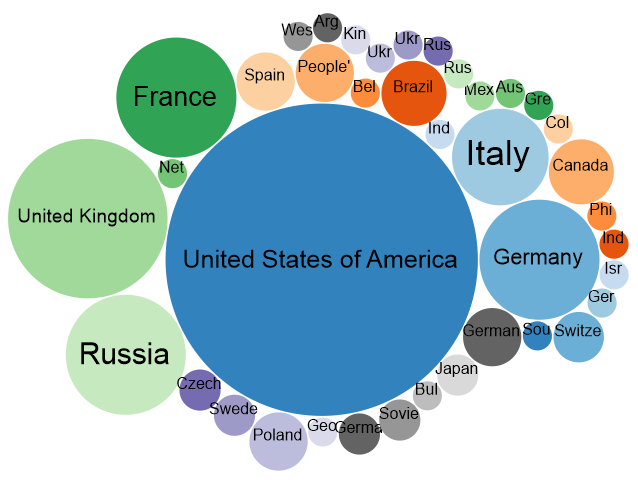
\includegraphics[width=0.7\textwidth]{./chapter/aircraft/Manufacture-with-country_2017.png}
	\caption{Соотношение количества производителей воздушных судов по странам, 2017 год.}
	\label{fig:Manufacture_with_country_2017}
\end{figure}

\label{aircraft_question_4}
\marginnote{
Как называется воздушное судно, удерживаемое в воздухе огромным баллоном с горючим смертельно опасным газом, расположенным прямо над головами пассажиров?
\\
См. ответ~\ref{answer:aircraft_question_airship} на с.~\pageref{answer:aircraft_question_airship}.
}

Как видно из ответа на запрос~\ref{lst:lang5} на рис.~\ref{fig:Manufacture_with_country_2017_2} указаны не все существующие производители воздушных судов, о чём свидетельствуют данные, взятые с сайта \href{https://www.aviationfanatic.com/}{aviationfanatic.com}. Более подробная информация о недостаточности данных в Викиданных даётся в следующем разделе этой главы. 
%Больше всего производителей указано у США (115), Великобритании (30), Германии (17), России (17) на 2017 год.

\begin{figure}[h!]
\centering
	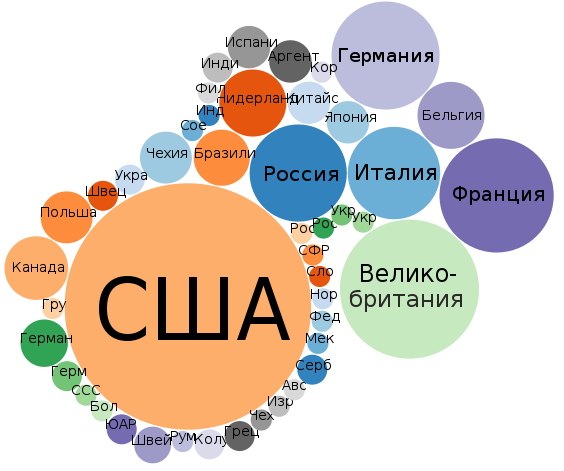
\includegraphics[width=0.7\textwidth]{./chapter/aircraft/Manufacture-with-country_2020.png}
	\caption{Соотношение количества производителей воздушных судов по странам, 2020 год.}
	\label{fig:Manufacture_with_country_2020}
\end{figure}

\label{fig:Manufacture_with_country_2017_2}

Сравнивая две пузырьковые диаграммы за 2017 (рис.~\ref{fig:Manufacture_with_country_2017}) и 2020 (рис.~\ref{fig:Manufacture_with_country_2020}) годы, можно сделать вывод, что основными производителями воздушных судов в мире 
в 2017 и 2020 годах были: США (115 заводов в 2017 и 135 заводов в 2020 году), Великобритания (30 и 43 завода), Германия (17 и 26 заводов) и Россия (17 и 21 завод). Лидером по-прежнему является США, а вот Франция за 3 года сумела опередить Германию, увеличив количество производств до 29 (Германия~--- 26), тем самым заняв третье место. Но в целом соотношение по производству воздушных судов между различными странами остаётся на прежнем уровне.

\section{Полнота Викиданных}

Согласно сайту \href{https://www.aviationfanatic.com/}{aviationfanatic.com} существует около \num{1700} производителей воздушных судов\cite{count_of_aircraft_manufactures} (2017 год) и \num{1939} (2020 год), но SPARQL-запрос~\ref{lst:lang2} вернул всего 300 авиазаводов в Викиданных в 2017 году, а в 2020 году~--- 595 авиазаводов. Из этого можно сделать вывод о неполноте Викиданных.  

\label{aircraft_question_5}
\marginnote{
Какое воздушное судно изображено на рис. \ref{fig:airship_question_aircraft}?
}


\begin{marginfigure}[0.0cm]
{
\setlength{\fboxsep}{0pt}%
\setlength{\fboxrule}{1pt}%
\fcolorbox{gray}{gray}{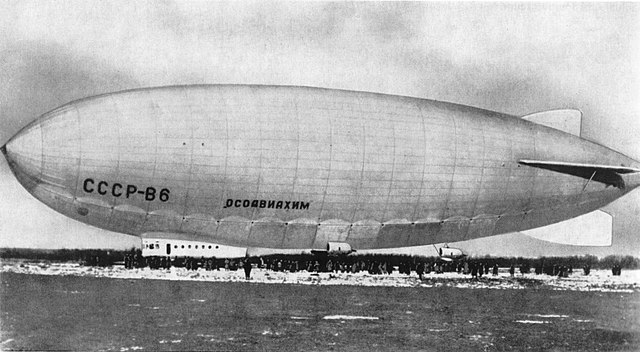
\includegraphics[width=\linewidth]{./chapter/aircraft/foto_of_airship.jpg}}%
}
  \caption{Неизвестное воздушное судно.}%
  \label{fig:airship_question_aircraft}%
\end{marginfigure}

\marginnote{

См. ответ~\ref{answer:aircraft_question_airship_2} на с.~\pageref{answer:aircraft_question_airship_2}.
}

Согласно приведённым выше данным можно сделать прогноз о том, когда Викиданные будут включать все данные сайта aviationfanatic.com. За три года количество производителей воздушных судов увеличилось на 239, что составляет ежегодный прирост примерно на 80 авиапроизводителей. Также за это время в Викиданные была занесена информация о 295 авиапроизводителях, то есть ежегодно добавляется около сотни авиазаводов. На 2020 год в Викиданных не было информации о \num{1344} авиапроизводителях, представленных на сайте \href{https://www.aviationfanatic.com/}{aviationfanatic.com}. Если считать, что ежегодно будет добавляться фиксированное количество новых авиапроизводителей и количество ежегодно заносимых записей в Викиданные останется неизменным, то можно предположить, что примерно через 75 лет (то есть в 2095 году) Викиданные будут содержать записи обо всех авиапроизводителях, представленных на сайте aviationfanatic.com.

\footnotetext{<<Авиастроительные компании России>>: \href{https://w.wiki/vF4}{https://w.wiki/vF4}}

В категории \href{https://cutt.ly/NhrKnWn}{<<Авиастроительные компании России>>} указано наличие в России 58 авиастроительных компаний в 2017 году и 62 завода, института и корпорации, связанных с самолётостроением, в 2020 году, но в то же время на сайте \href{https://www.aviationfanatic.com/}{aviationfanatic.com} указано наличие 61 завода\cite{count_plants_of_aircrafts} в 2017 году и 71 в 2020 году. Среди авиастроительных компаний России представлены такие компании как: \href{https://clck.ru/RxFCs}{Иркут}, \href{https://clck.ru/QR6qZ}{МиГ}, \href{https://clck.ru/RxFG3}{Туполев}.

%\section{Степень заполненности Викиданных}

%Для заполнения были выбраны поля label и description у объектов, перечисленных в категории <<Авиастроительные компании России>>. Так как объектов там много, было решено автоматизировать заполнение, для чего была написана соответствующая программа. Для начала был создан JSON-файл с объектами из категории и пустыми полями для заполнения:

%\begin{lstlisting}[ language=SPARQL, label=lst:lang6, ]
%{
%  "121 авиационный ремонтный завод": {
%    "description": "",
%    "descriptionen": "",
%    "nameen": "",
%    "qid": "Q4028573"
%    },
%  ...
%}
%\end{lstlisting}

%В первой части программы записывались уже существующие значения полей из Викиданных в JSON-файл. После чего было необходимо заполнить оставшиеся пустыми поля, то есть поля, не заполненые в Викиданных. В итоге JSON-файл выглядел примерно так:

%\begin{lstlisting}[ language=SPARQL, label=lst:lang7, ]
%{
%  "121 авиационный ремонтный завод": {
%    "description": "авиаремонтное предприятие, расположенное посёлке Старый Городок",
%    "descriptionen": "aircraft repair facility, located in the village Stary Gorodok",
%    "nameen": "121 aircraft repair plant",
%    "qid": "Q4028573"
%  },
%  ...
%}
%\end{lstlisting}

%Во второй части программы записывались данные из JSON-файла в Викиданные.

%С помощью этой программы удалось упростить работу с Викиданными, так как не приходилось самостоятельно заходить на страницы объектов и вносить изменения, если существующие данные не удовлетворяют ожиданиям, то есть поле в Викиданных отличается от локального.

\section{Упражнения}
\begin{enumerate}
\item Найти самолет с максимальным радиусом полета.
\item Отметить на политической карте мира местоположение главных офисов компаний авиапроизводителей.
\item Найти производителя с максимальным числом изготовленных самолетов, используя свойство \href{https://w.wiki/vF7}{\textit{manufacturer (P176)}} у воздушных судов.
\item Когда был построен первый самолёт?
\item Какие фирмы первыми выпустили 10, 100 и тысячу самолётов?
\item Нарисуйте диаграмму количества выпускаемых самолётов в мире и в России по годам.
\end{enumerate}
